\section{Experimental overview of Bottomonia results in heavy ion collisions}

\subsection{$\Upsilon$(nS) Nuclear Modification Factor R$_{AA}$}
A large set of heavy ion collisions data is available at both RHIC and LHC energies.
RHIC at BNL is designed for Au+Au collisions
at $\sqrt{s_{\rm NN}}$ = 200 GeV and can accelerate ions upto Uranium. Both PHENIX and
STAR experiments at RHIC can measure quarkonia in dimuon channel. 
LHC runs part of the time for heavy ion program and it
can perform PbPb collision upto $\sqrt{s_{\rm NN}}$ = 5.5 TeV. In addition, d+Au collisions
are performed at RHIC and pPb collisions are performed at LHC to study
intermediate system. The CMS. ATLAS and ALICE detectors at LHC have obtained large
amount of Upsilon data in different kinematic ranges.

To quantify the effect of medium in the quarkonia production scenario one takes
recourse to a quantity called the nuclear modification factor $(R_{AA})$. This quantity
is defined as the ratio of the quarkonium yield in the A-A collisions to the same
in case of p-p collisions scaled by the number of collisions : 
 \begin{equation}
 R_{AA} = \frac{1}{\langle N_{coll} \rangle} \ \frac {N^{Q{\bar Q}}_{AA}} {N^{Q{\bar Q}}_{pp}} 
 \end{equation}
 The ratio will be unity if the physics of the A-A collisions is simply the sum of
 a scaled number p-p collisions. The effect of the medium should make it vary from unity. 
In this section, we review the current status of the experimental measurement
of nuclear modification factor ($R_{\rm AA}$) and elliptic flow ($v_{2}$) of the
$\Upsilon$ states. The results from different experiments are compared to
understand effects of the medium and their dependence on the collision energy
and kinematic ranges. 



\paragraph{Measurement by CMS, ATLAS and ALICE}
 The cross sections of bottomonia at LHC are large and hence all the 
bottomonia states ($\Upsilon$(nS)) are measured at the LHC with very good statistical
precision~\cite{Chatrchyan:2011pe,Chatrchyan:2012lxa,Abelev:2014nua,Khachatryan:2016xxp}.
 PbPb collisions at LHC were performed at $\sqrt{s_{\rm NN}}$ = 2.76 TeV staring from 
2011. pp collisions were performed at the same energy and pPb collisions were performed
at $\sqrt{s_{\rm NN}}$ = 5.02 TeV. 
During second LHC run, PbPb collisions were perfomed at $\sqrt{s_{\rm NN}}$ = 5.02 TeV 
and pPb collisions were perfomred at $\sqrt{s_{\rm NN}}$ = 8 TeV. 
The CMS experiment can reconstruct all the three states of Upsilon staring from
$p_T$=0 covering a large range in central region with rapidity $|y| < 2.4$.
ALICE experiment can reconstruct Upsilon in the forward rapidity range
$2.5 < y < 4.0$ in muon arm.
The reach of ATLAS experiment is within $|y| < 1$ but it can measure upto high $p_T$.
At lower energy, STAR experiment can reconstruct in mid-rapidty range
$|y| < 1.0$ from zero $p_T$ onwards. 

\begin{figure}
  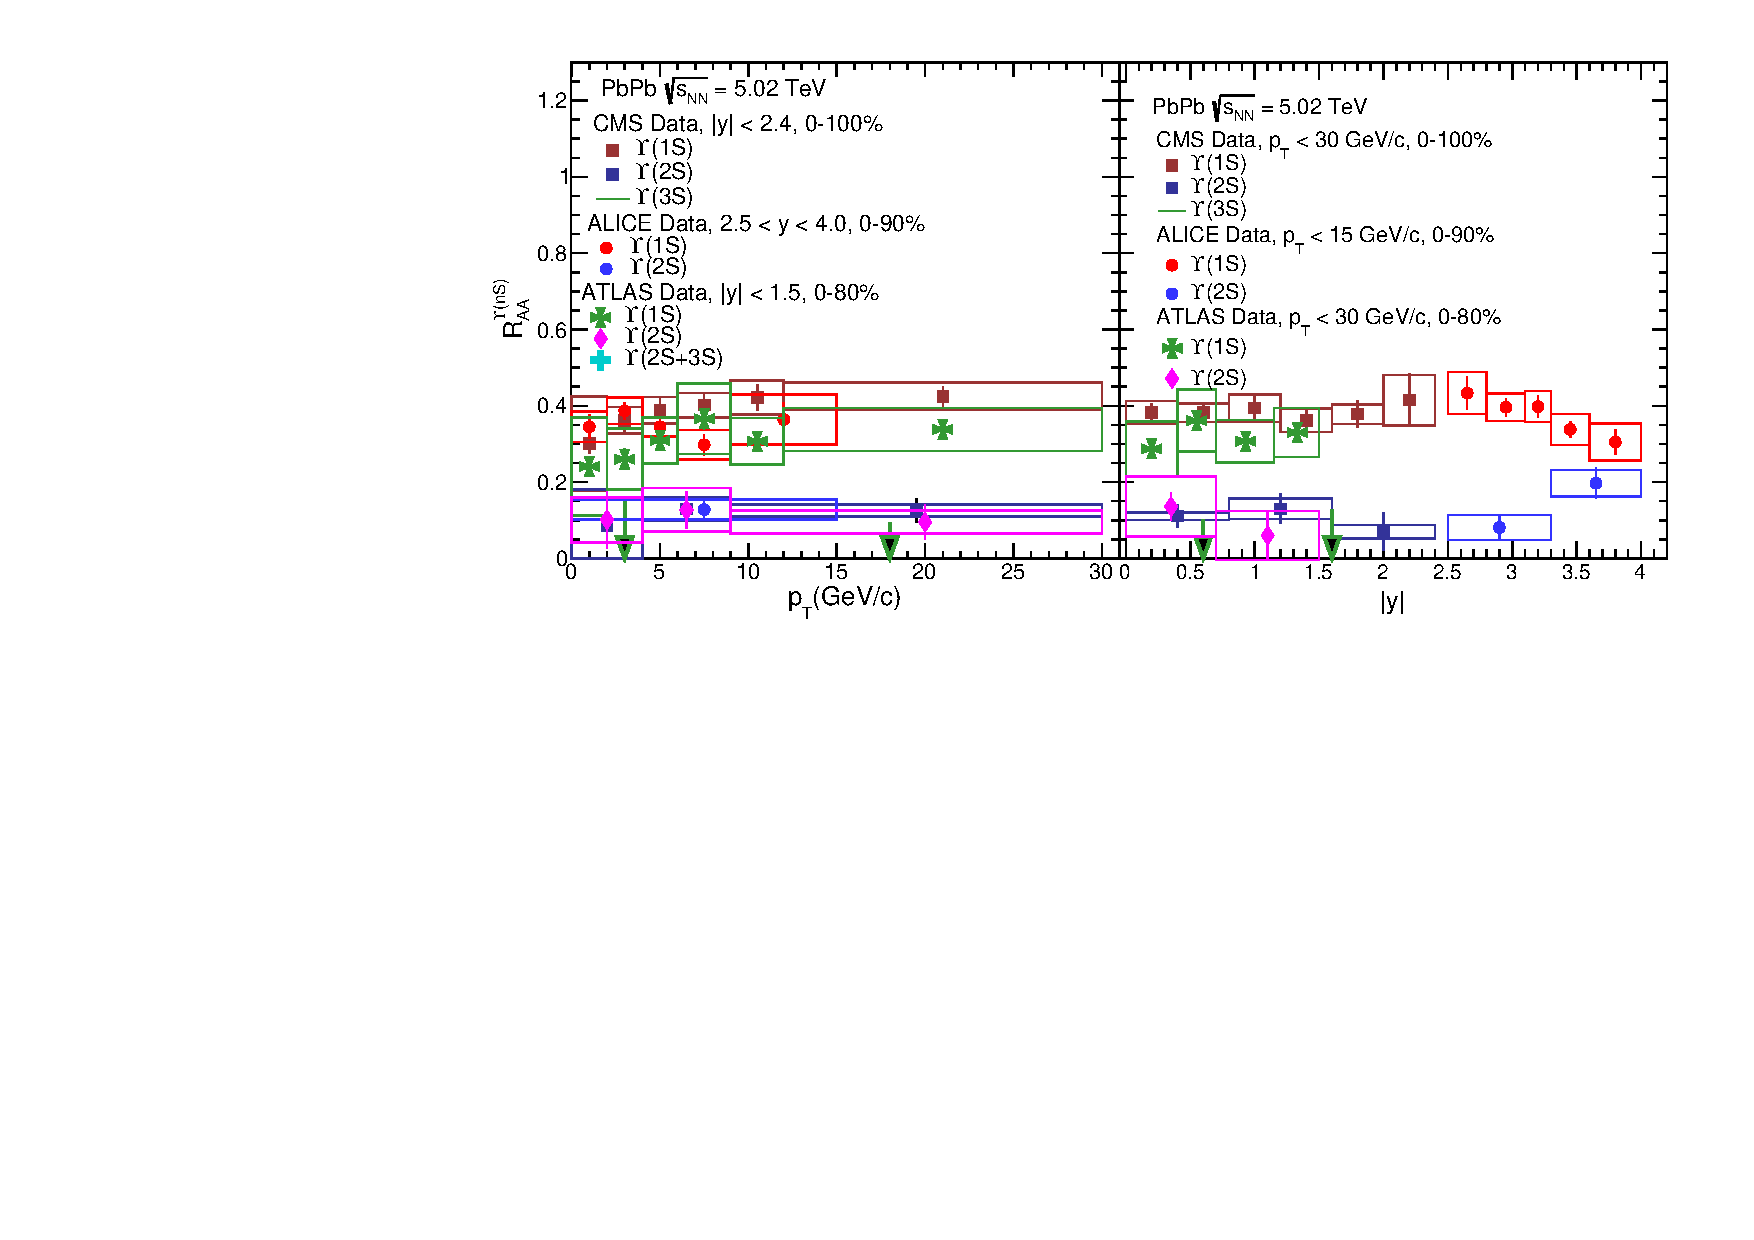
\includegraphics[width=0.99\textwidth]{Figures/Fig5_LHC_YnSRAAPtRap.pdf}
  \caption{(Color online) The $\Upsilon$(nS) nuclear modification factor, $R_{AA}$
in PbPb collisions at $\sqrt{s_{\rm NN}}$ = 5.02 TeV, (a) as a function of transverse momentum $p_{T}$
    and (b) as a function of rapidity measured by CMS~\cite{CMS:2018zza}, ALICE~\cite{ALICE:2020wwx}
    and ATLAS experiments~\cite{ALICE:2020wwx}.
    The vertical bars denote statistical uncertainties, and the rectangular boxes
    show the total systematic uncertainties.
  }
  \label{fig:LHCYnSRAAPtRap}
\end{figure}


\begin{figure}
  \begin{center}
  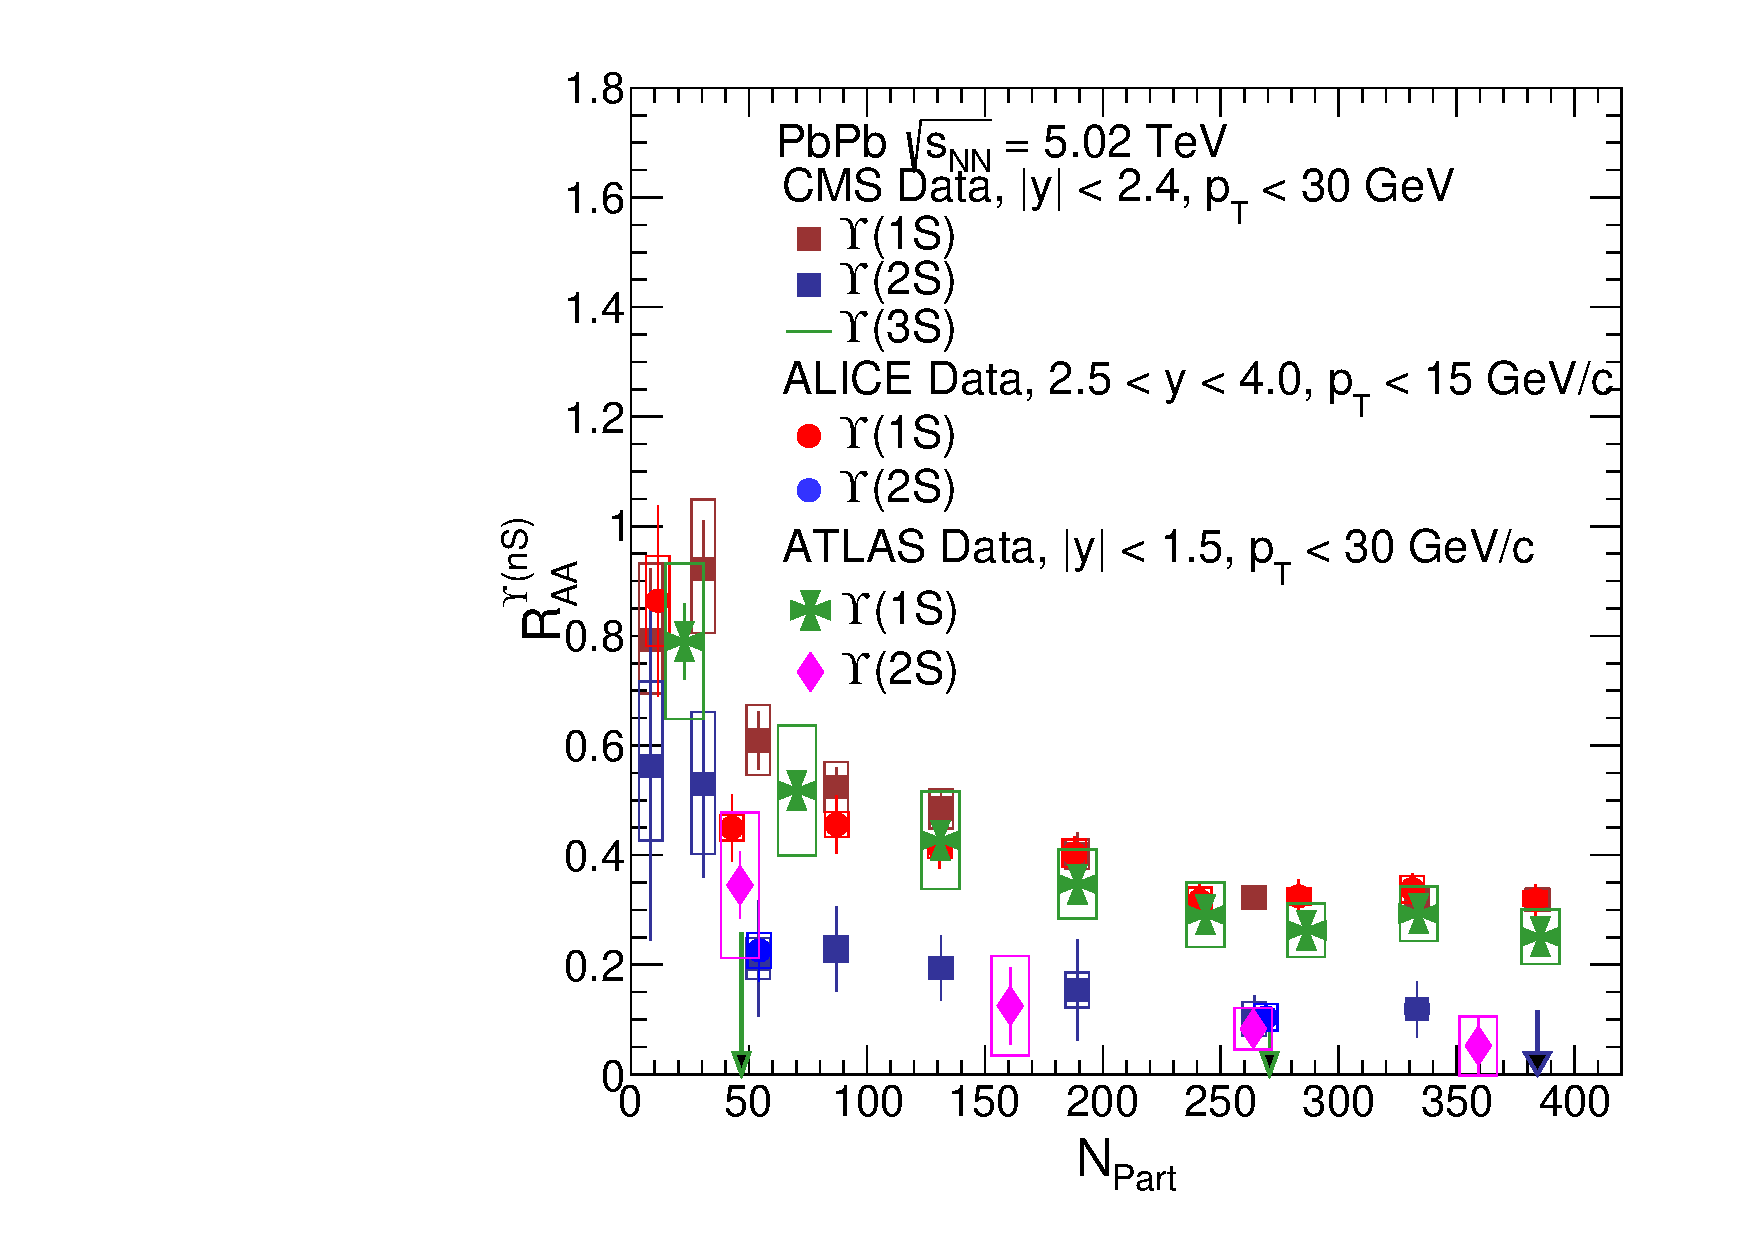
\includegraphics[width=0.6\textwidth]{Figures/Fig6_LHC_YnSRAANPart.pdf}
  \caption{(Color online) The $\Upsilon$(nS) nuclear modification factor, $R_{AA}$
   in PbPb collisions at $\sqrt{s_{\rm NN}}$ = 5.02 TeV as a function of $N_{\rm Part}$
   measured by CMS~\cite{CMS:2018zza}, ALICE experiments~\cite{ALICE:2020wwx} and
   ATLAS experiments~\cite{ALICE:2020wwx}.
   The vertical bars denote statistical uncertainties and the rectangular boxes show
   the total systematic uncertainties.
  }
  \label{fig:LHCYnSRAANPart}
  \end{center}
\end{figure}



\begin{figure}
  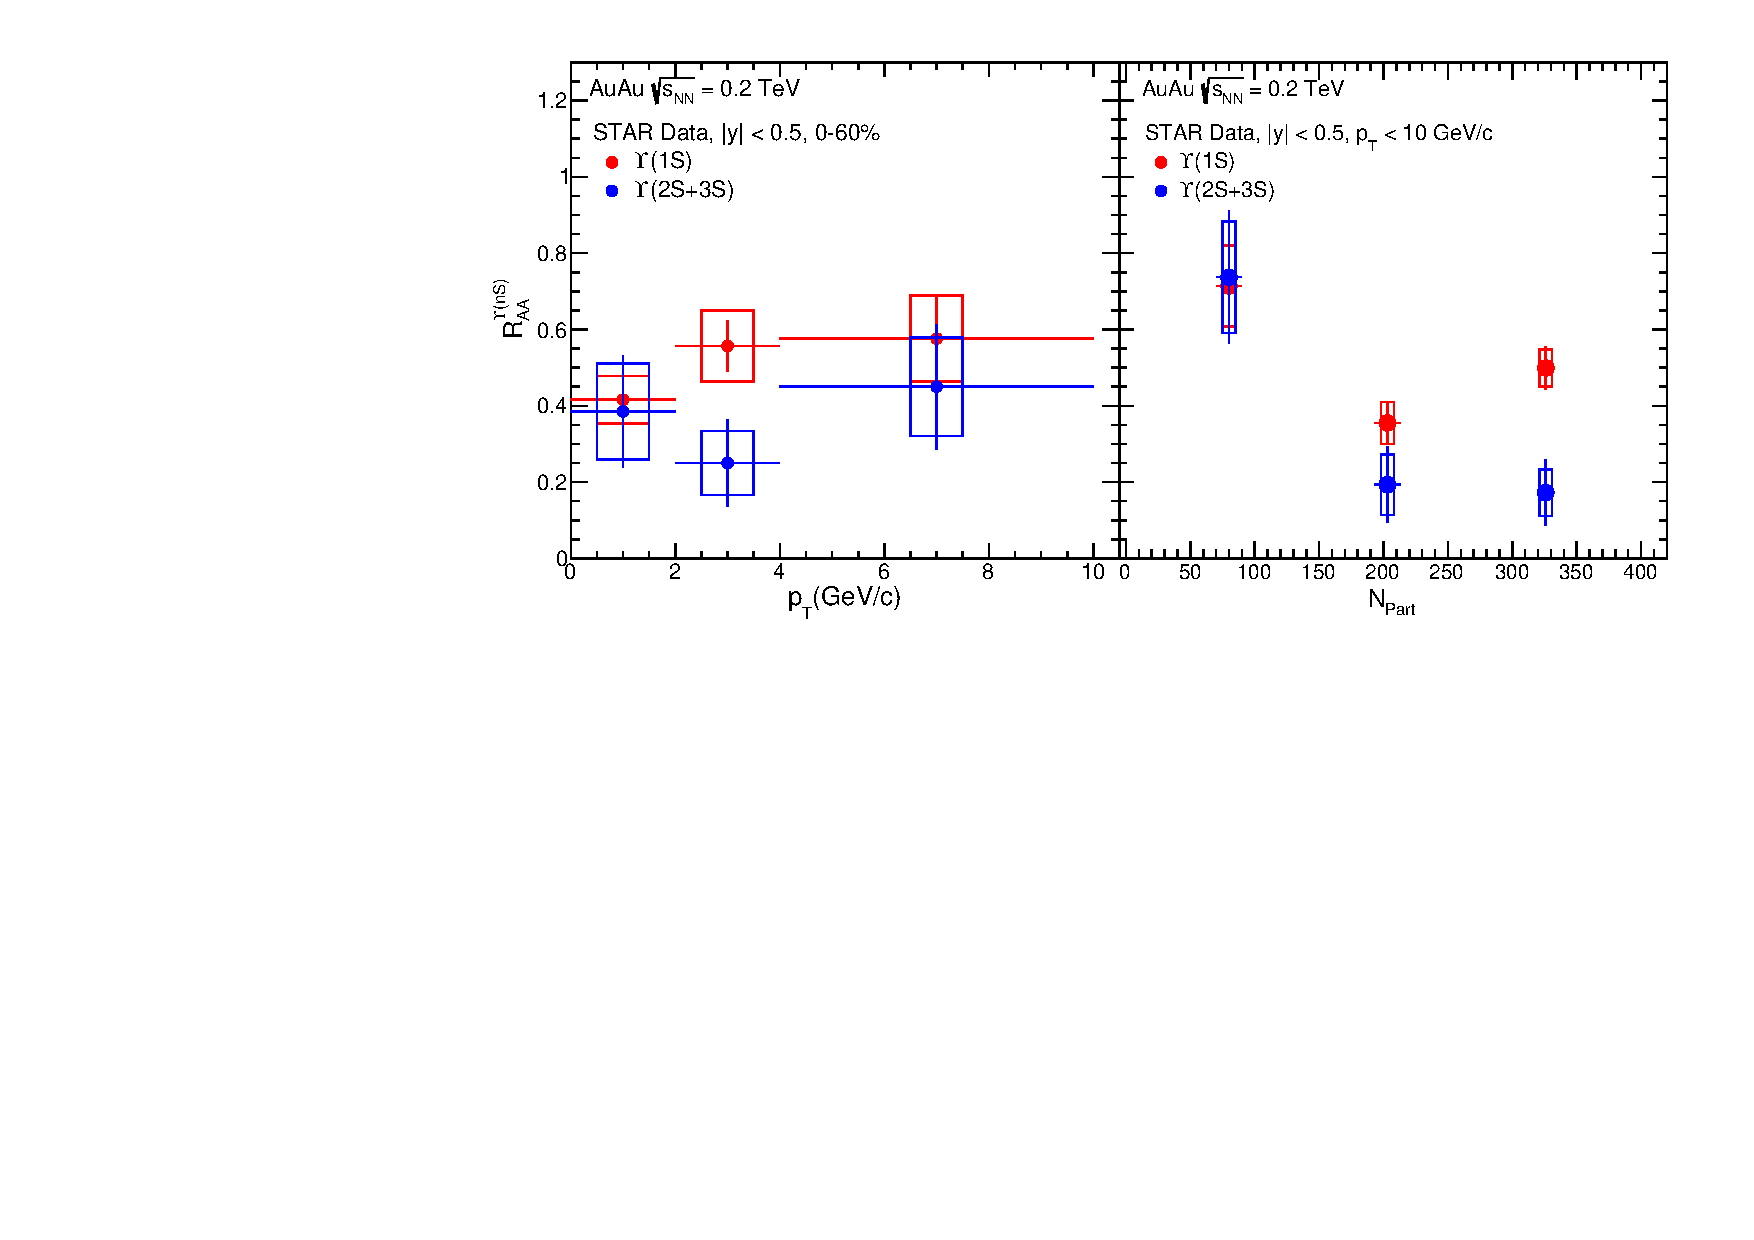
\includegraphics[width=0.99\textwidth]{Figures/Fig7_RHIC_YnSRAAPt.pdf}
  \caption{(Color online) The $\Upsilon$(nS) nuclear modification factor, $R_{AA}$
in AuAu collisions at $\sqrt{s_{\rm NN}}$ = 200 GeV,
     (a) as a function of transverse momentum $p_{T}$
    and (b) as a function of $N_{\rm Part}$ measured by STAR experiments~\cite{Wang:2019vau}. The vertical bars denote
    statistical uncertainties, and the rectangular boxes show the total systematic uncertainties.
  }
  \label{fig:RHICYnSRAAPt}
\end{figure}



\begin{figure}
  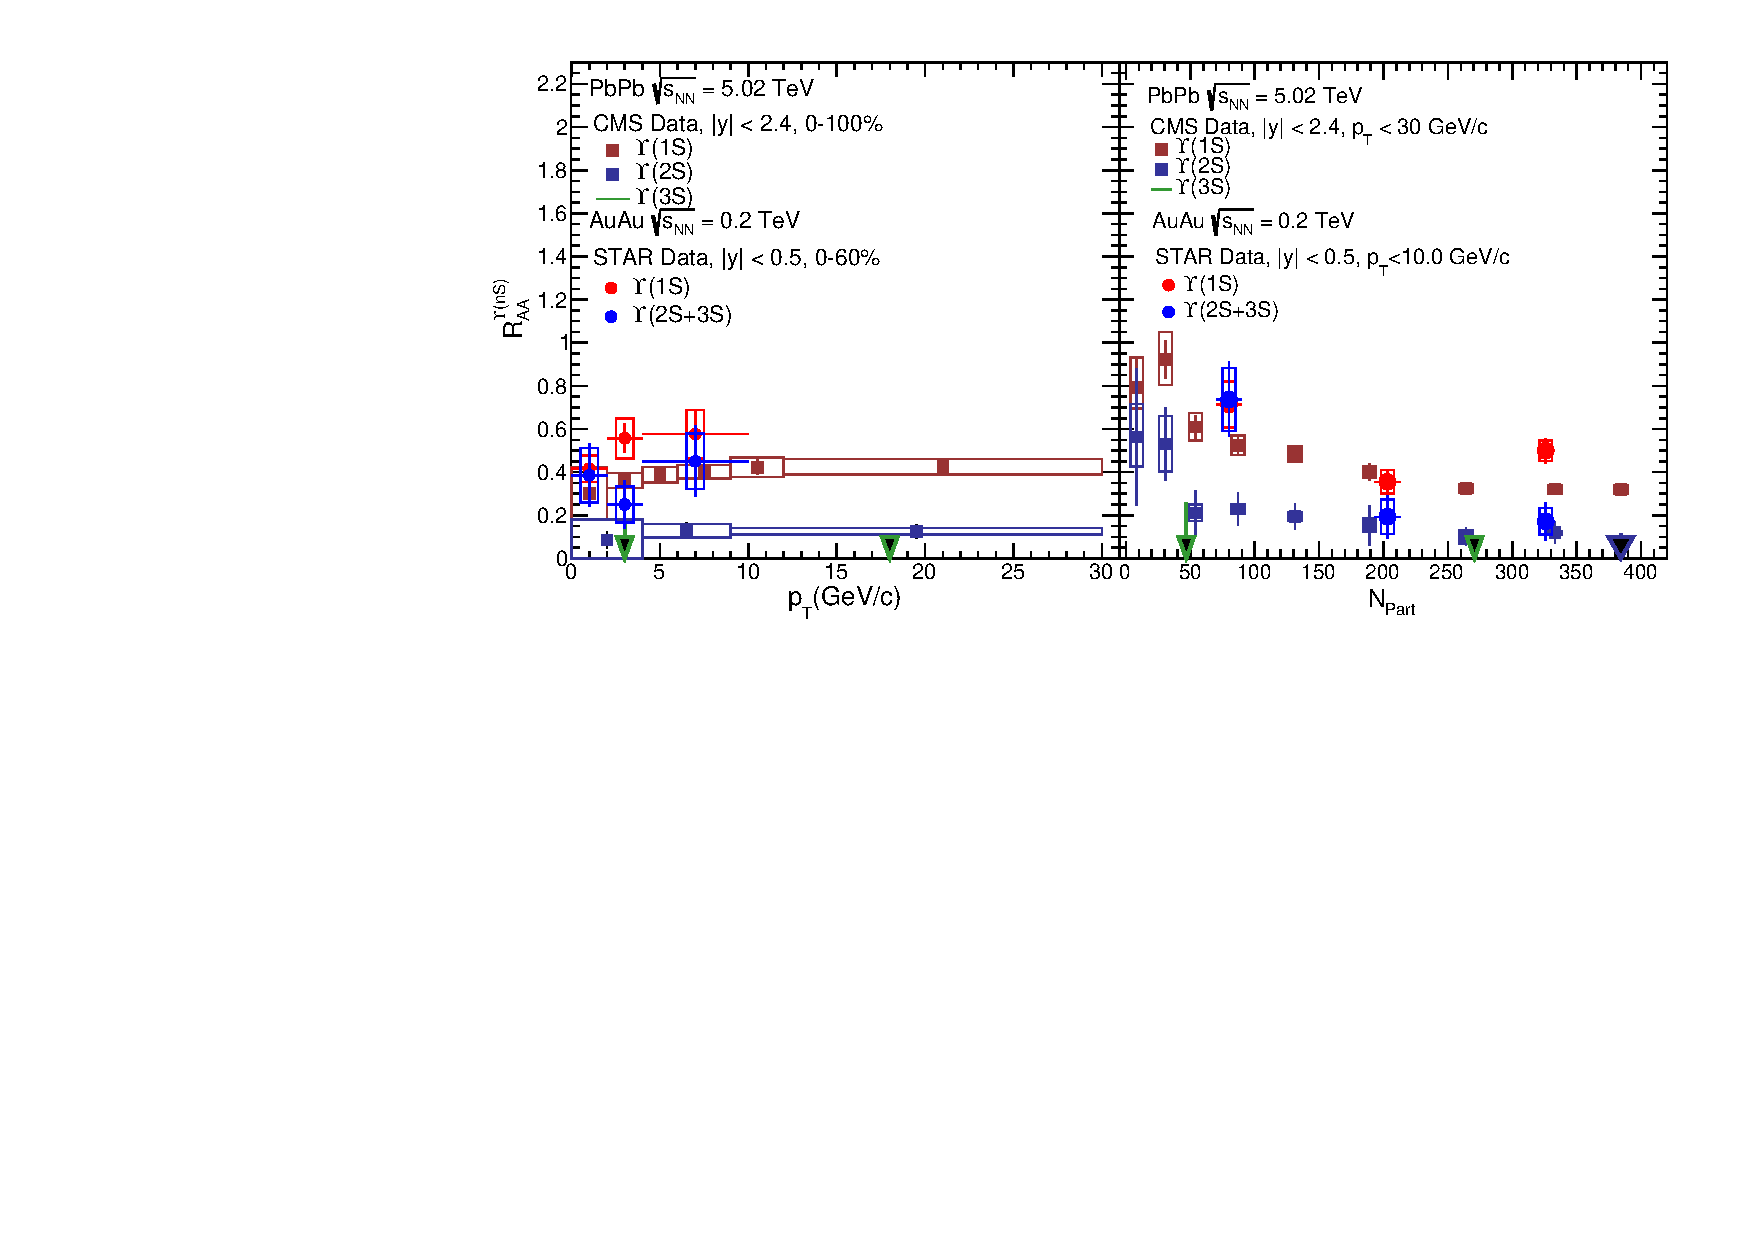
\includegraphics[width=0.99\textwidth]{Figures/Fig8_RHIC_LHC_YnSRAA.pdf}
  \caption{(Color online) The $\Upsilon$(nS) nuclear modification factor, $R_{AA}$, (a) as a function of transverse momentum $p_{T}$
    and (b) as a function of $N_{\rm Part}$ measured by STAR experiments~\cite{Wang:2019vau} at 0.2 TeV and CMS experiment~\cite{CMS:2018zza} at 5.5 TeV.
    The vertical bars denote statistical uncertainties, and the rectangular boxes show the total systematic uncertainties.
  }
  \label{fig:RHICYnSRAANPart}
\end{figure}


Figure~\ref{fig:LHCYnSRAAPtRap} shows the $\Upsilon$(nS) nuclear modification factor, $R_{AA}$
in PbPb collisions at $\sqrt{s_{\rm NN}}$ = 5.02 TeV, (a) as a function of transverse momentum $p_{T}$
and (b) as a function of rapidity measured by CMS~\cite{CMS:2018zza}, ALICE~\cite{ALICE:2020wwx}
and ATLAS experiments~\cite{ALICE:2020wwx}.
 The vertical bars denote statistical uncertainties, and the rectangular boxes
show the total systematic uncertainties. From these figures it is clear 
that the individual $\Upsilon$ states are suppressed in
the PbPb collisions relative to the production in the pp collisions.
One can also notice that $\Upsilon$(2S) and $\Upsilon$(3S) are 
more suppressed relative to the ground state $\Upsilon$(1S) and there is sequential
suppression pattern as per the binding energies of the states.
$\Upsilon$(3S) almost disappears in PbPb collisions. 
The suppression of $\Upsilon$ states increases with $\pT$ and $R_{AA}$ looks
to be flat at high $p_T$
although more precise measurements (at high $p_T$) are required to ascertain
this behaviour. 
With increasing rapidity, the suppression remains the same and decreases
slightly but only at larger rapidities.
The forward rapidity ($2.5 \leq y^{\Upsilon} \leq 4.0$) measurement of the $\Upsilon$ suppression at 
ALICE is found to be consistent with the midrapidity ($|y^{\Upsilon}|\,\leq 2.4$)
measurement of the $\Upsilon$ suppression at the CMS which again shows the weak dependence
of suppression on rapidity.



Figure~\ref{fig:LHCYnSRAANPart} shows
the $\Upsilon$(nS) nuclear modification factor, $R_{AA}$
in PbPb collisions at $\sqrt{s_{\rm NN}}$ = 5.02 TeV, as a function of $N_{\rm Part}$
measured by CMS~\cite{CMS:2018zza}, ALICE experiments~\cite{ALICE:2020wwx}
and ATLAS experiments~\cite{ALICE:2020wwx}.
 The vertical bars denote statistical uncertainties and the rectangular
boxes show the total systematic uncertainties. The $\Upsilon$ nuclear modification
factor, $R_{AA}$, shows a strong dependence on collision centrality and the
suppression of all the states increases as the collisions become more central
corresponding to bigger system size. 

    
Figure~\ref{fig:RHICYnSRAAPt} shows the $\Upsilon$(nS) nuclear modification factor, $R_{AA}$
in AuAu collisions at $\sqrt{s_{\rm NN}}$ = 200 GeV,
 (a) as a function of transverse momentum $p_{T}$
and (b) as a function of $N_{\rm Part}$ measured by STAR
experiments~\cite{Wang:2019vau}. The vertical bars denote
statistical uncertainties, and the rectangular boxes show the total systematic
uncertainties. At RHIC energy the suppression pattern of Upsilon states
looks similar as we discussed for LHC; Higher states are more suppressed,
the suppression has weak dependence on $p_T$ and strong dependence on $N_{\rm part}$.



Figure~\ref{fig:RHICYnSRAANPart} shows
  the $\Upsilon$(nS) nuclear modification factor, $R_{AA}$, (a) as a function of transverse momentum $p_{T}$
  and (b) as a function of $N_{\rm Part}$ measured by STAR experiments~\cite{Wang:2019vau} at $\sqrt{s_{\rm NN}}$ =0.2 TeV and
  CMS experiment~\cite{CMS:2018zza} at $\sqrt{s_{\rm NN}}$ =5.5 TeV.
The vertical bars denote statistical uncertainties, and the
rectangular boxes show the total systematic uncertainties.
One can note that the suppression of Upsilon states is slightly stronger at
LHC as compared to that at RHIC.   


  


\begin{figure}
  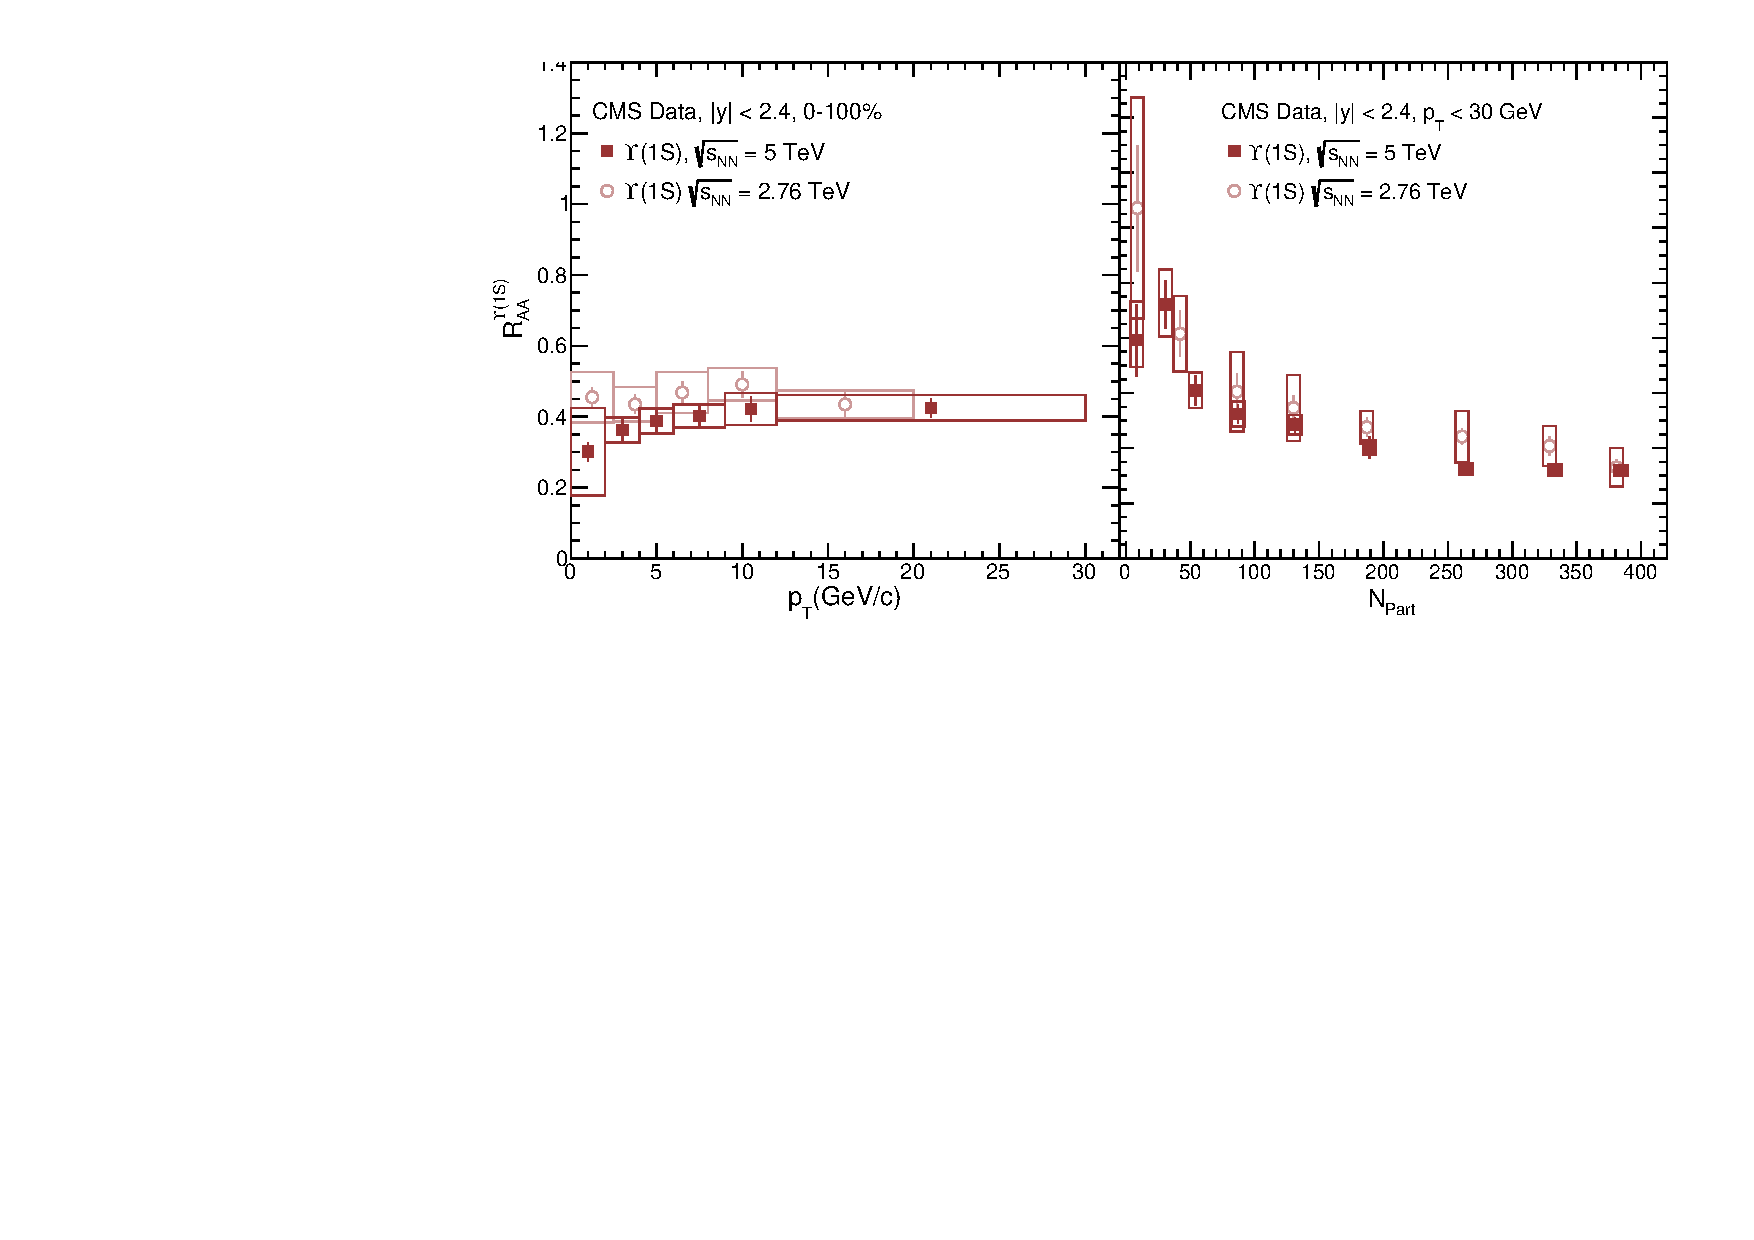
\includegraphics[width=0.99\textwidth]{Figures/Fig9_CMS_Y1SRAAPtNPart_En.pdf}
  \caption{(Color online) The $\Upsilon$(nS) nuclear modification factor, $R_{AA}$ in PbPb collisions,
    (a) as a function of transverse momentum $p_{T}$
    and (b) as a function $N_{\rm Part}$ measured by CMS 
    at 2.76~\cite{Khachatryan:2016xxp} and 5.02 TeV~\cite{CMS:2018zza}
  }
  \label{fig:LHCYnSRAAenergy}
\end{figure}




Figure~\ref{fig:LHCYnSRAAenergy} shows 
the $\Upsilon$(nS) nuclear modification factor, $R_{AA}$ in PbPb collisions,
(a) as a function of transverse momentum $p_{T}$
  and (b) as a function $N_{\rm Part}$ measured by CMS
    at 2.76~\cite{Khachatryan:2016xxp} and 5.02 TeV~\cite{CMS:2018zza}. 
 The CMS experiment measured slightly more amount of $\Upsilon$ suppression at
 $\sNN =$ 5.02 TeV than the suppression at $\sNN =$ 2.76 TeV.
 The ALICE experiment on the other hand observed less
suppression at $\sNN =$ 5.02 TeV than that at $\sNN =$ 2.76 TeV 
in the most central PbPb collisions~\cite{ALICE:2018wzm,Abelev:2014nua}. 
  
Overall, LHC provided high statistics measurements of all three
Upsilon states over wide kinematical ranges. At high $p_T$ more precise
measurements are required to ascertain flatness in the suppression. 


    
    
\subsection{$\Upsilon$(nS) azimuthal anisotropy}


In semi-central heavy ion collisions,
the produced QGP has a lenticular shape in the transverse plane
which is reflected in the anisotropic
distribution of particles obtained using the magnitudes
of the Fourier co-efficients ($v_{n}$) of the azimuthal correlation of
particles~\cite{Voloshin:1994mz}. By studying the azimuthal distribution of
the quarkonia, it is possible to develop a more comprehensive understanding
of the dynamics of their production.

\begin{figure}
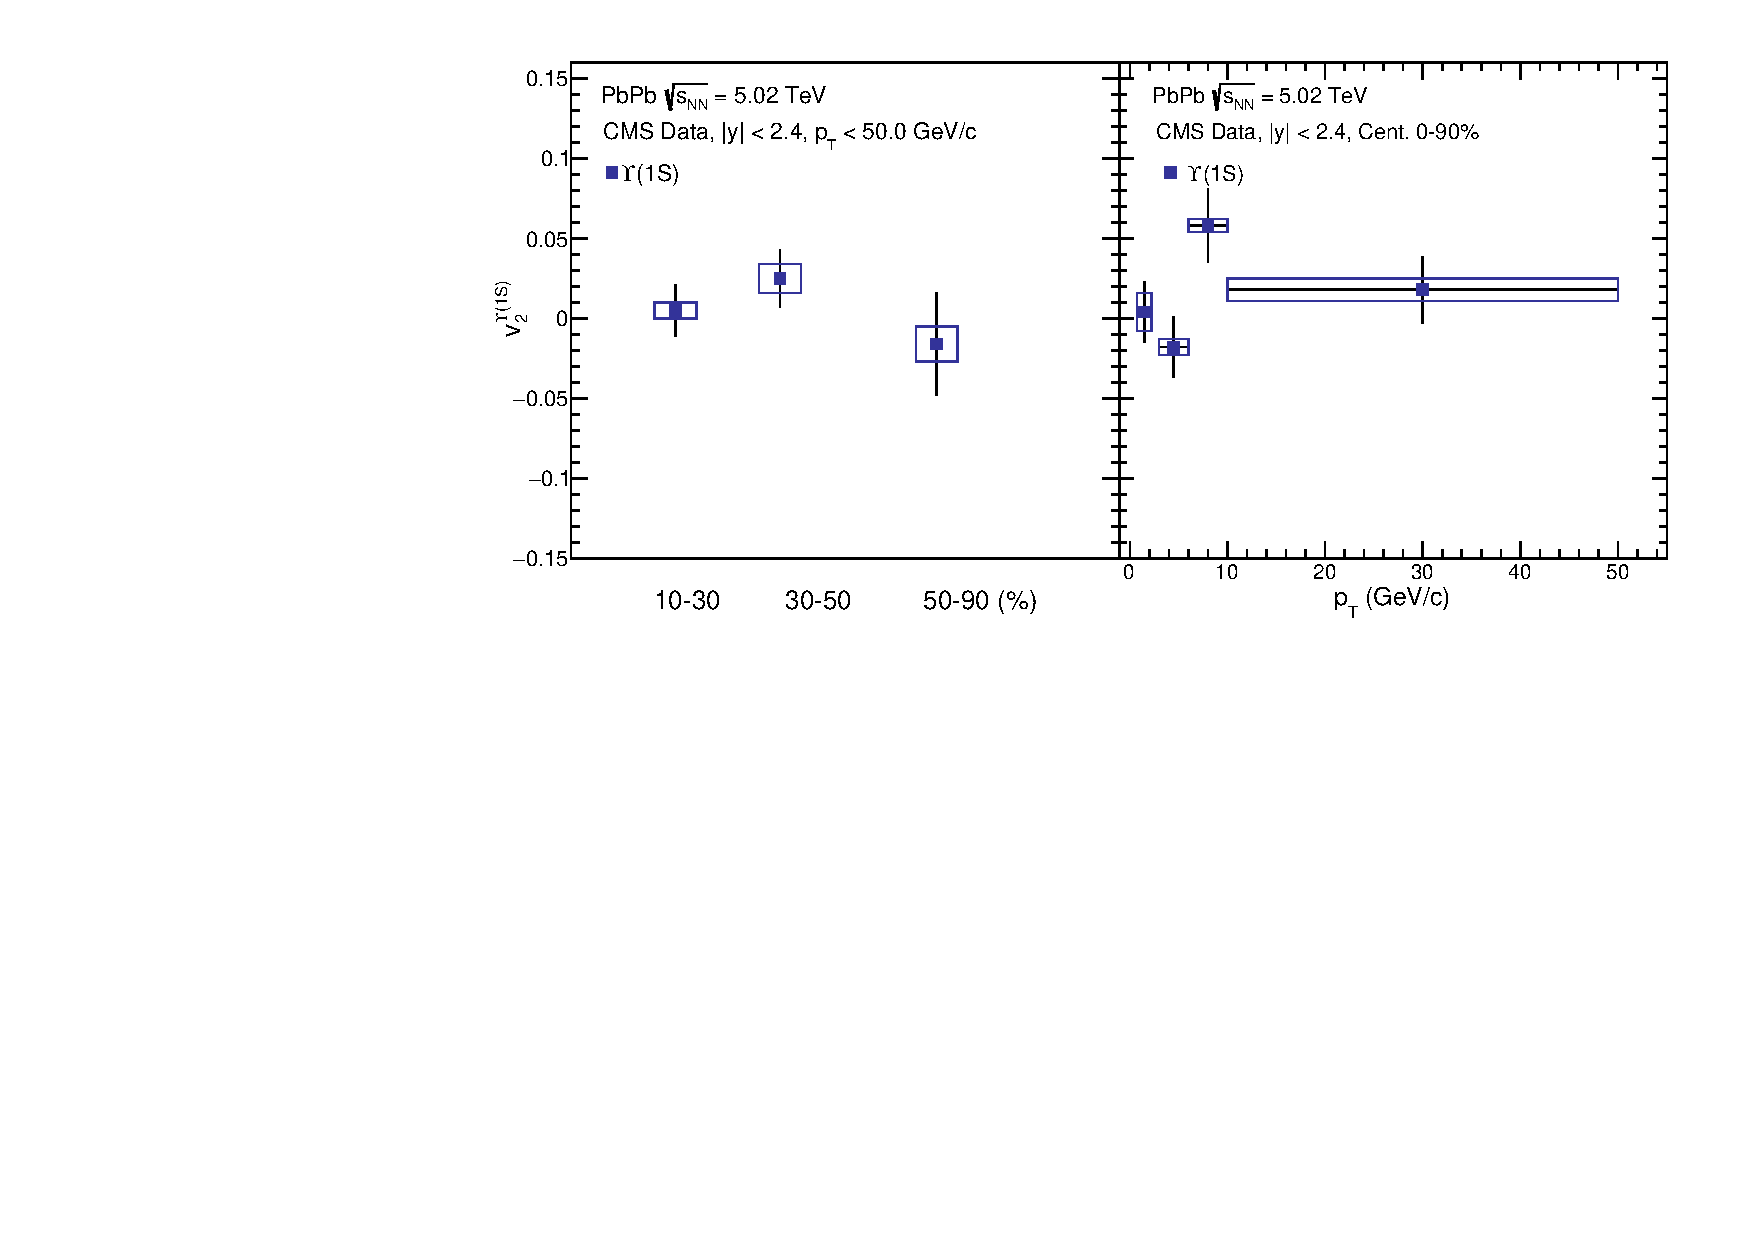
\includegraphics[width=0.99\textwidth]{Figures/Fig10_CMS_Y1S_5TeV_V2.pdf}
\caption{(Color online) The $\Upsilon$(1S) azimuthal anisotropy ($v_{2}$) (a) as a
  function of collision centrality and (b) as a function of transverse momentum
  $p_{T}$~\cite{CMS:2020efs}. The vertical bars denote statistical uncertainties,
  and the rectangular boxes show the total systematic uncertainties.
}
\label{fig:Upsilon1SV2CMS}
\end{figure}



The CMS experiment measured $v_{2}$ coefficients for $\Upsilon$(1S) and $\Upsilon$(2S)
mesons in PbPb collisions at $\sqrt{s_{NN}}=$ 5.02 TeV.
Figure~\ref{fig:Upsilon1SV2CMS} shows the $\Upsilon$(1S) azimuthal
anisotropy ($v_{2}$) (a) as a function of collision centrality and (b) as a
function of transverse momentum $p_{T}$ measured by CMS experiment at
LHC~\cite{CMS:2020efs}. The p$_{T}$ integrated results shown in
Fig.~\ref{fig:Upsilon1SV2CMS} (a) for three centrality intervals are consistent
with zero within the statistical uncertainties. The average $v_{2}$ values in the
10-90$\%$ centrality interval measured by CMS experiment are found to
be 0.007$\pm$0.011(stat)$\pm$0.005(syst) for $\Upsilon$(1S) and
-0.063$\pm$0.085(stat)$\pm$0.037(syst) for $\Upsilon$(2S).   
The p$_{T}$ dependence of $\Upsilon$(1S) meson $v_{2}$ values is measured
for the 10-90$\%$ centrality interval. The values of $v_{2}$ are consistent with
zero in the measured p$_T$ range, except for the 6$<$p$_T$$<$10 GeV/c interval that
shows a 2.6$\sigma$ deviation from zero. 

\begin{figure}
  \begin{center}
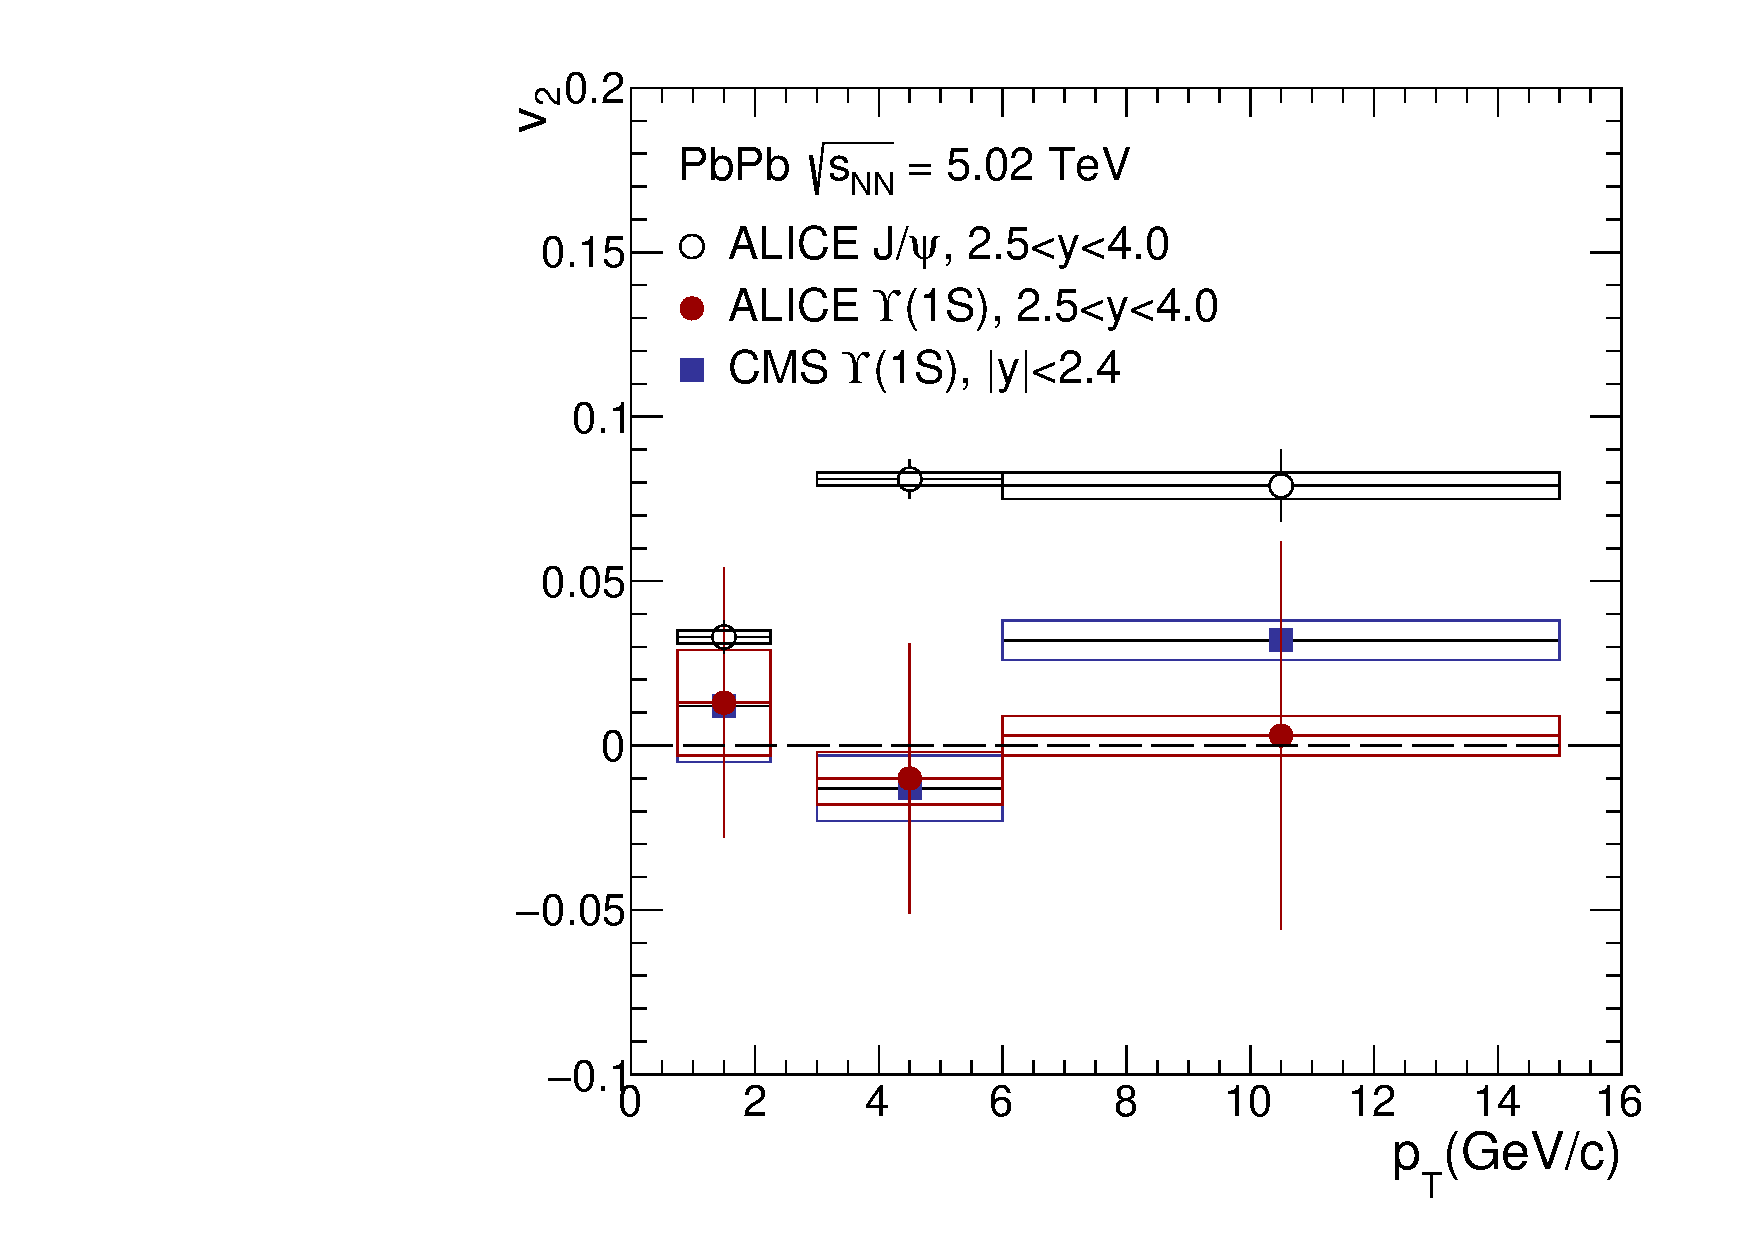
\includegraphics[width=0.6\textwidth]{Figures/Fig11_CMS_ALICE_Y1S_5TeV_V2.pdf}
\caption{(Color online) The $v_{2}$ for $\Upsilon$(1S) mesons as a function of p$_{T}$ in the
  rapidity range $|y|<2.4$ measured by
  CMS experiment~\cite{CMS:2020efs} compared with the ALICE results for $Upsilon$(1S)
  and J/$\psi$ mesons measured in 2.5$<$y$<$4~\cite{ALICE:2019pox}.
  The vertical bars denote statistical uncertainties,
  and the rectangular boxes show the total systematic uncertainties.
}
\label{fig:Upsilon1SV2Compare}
\end{center}
\end{figure}

Figure~\ref{fig:Upsilon1SV2Compare} shows the p$_{T}$ differential results
for $v_{2}$ of $\Upsilon$(1S) mesons measured by CMS experiment along with the
measurements of $v_{2}$ for $\Upsilon$(1S) and J/$\psi$ from ALICE in the same
p$_{T}$ (0-15 GeV/c) and centrality (5-60$\%$) interval. The measurements from CMS
and ALICE are done in complementary rapidity ranges. The $\Upsilon$(1S) $v_{2}$ is
consistant with zero while the J/$\psi$ meson measured by ALICE in same kinematic
conditions has finite $v_{2}$. Together, the CMS and ALICE
results indicate that the collective effects of the medium on the 
$\Upsilon$(1S) are small.



\subsection{$\Upsilon$(nS) in proton Lead collisions }

The CMS experiment measured the $\Upsilon$ ratios as a function of event activity  
in pPb collisions at $\sqrt{s_{NN}}$=5.02 TeV~\cite{CMS:2013jsu}.
The results were compared with pp and PbPb collisions at $\sqrt{s}$=2.76 TeV.
 The nuclear modification of all $\Upsilon$ states is also measured in pPb collisions
 at $\sqrt{s_\mathrm{NN}}$ = 5.02 TeV~\cite{CMS:2022wfi}.
 Recently, relative production of $\Upsilon$(nS) states are measured as a function of
 event activity in proton-proton collisions at $ \sqrt{s} $ = 7 TeV~\cite{CMS:2020fae}.

   



\begin{figure}
  \begin{center}
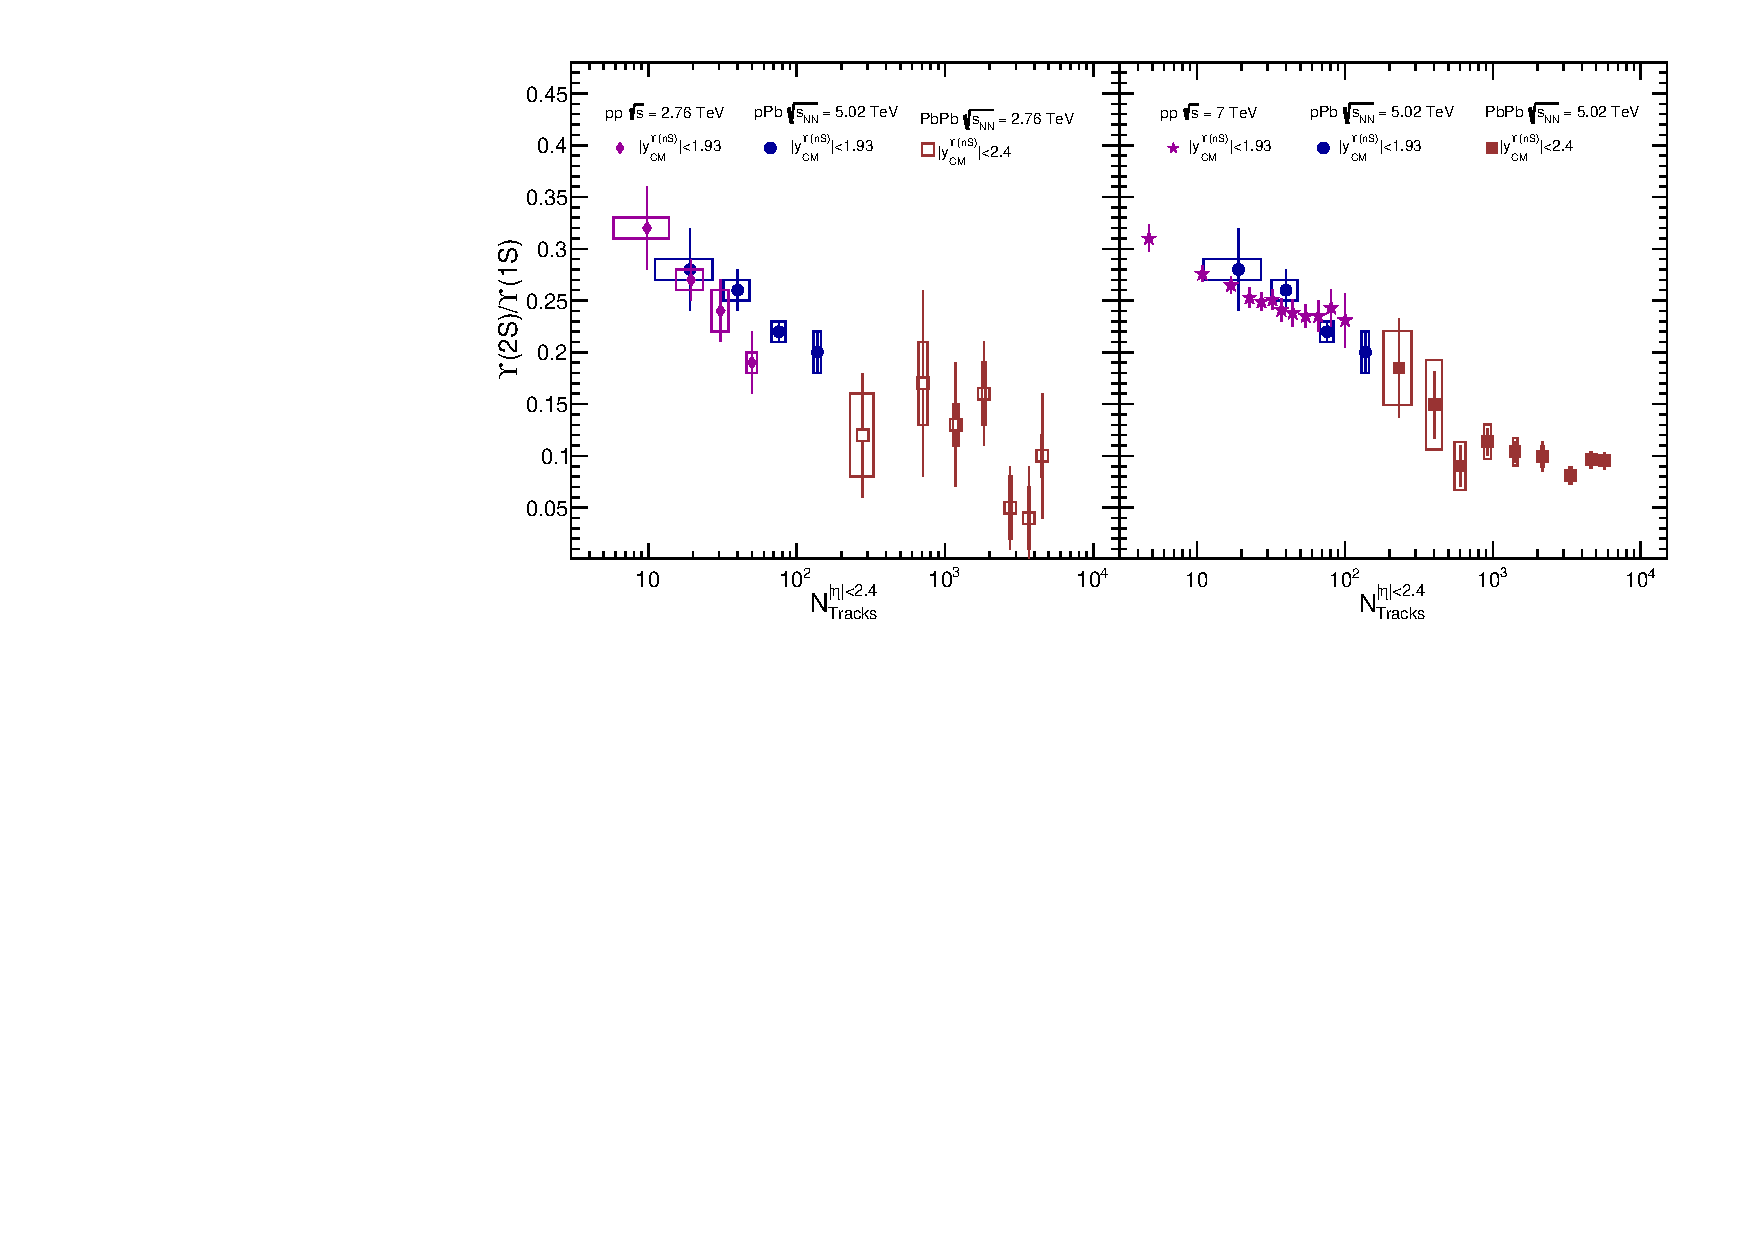
\includegraphics[width=0.99\textwidth]{Figures/Fig12_LHC_Y2SByY1S_NTrk.pdf}
\caption{(Color online)
  (a) The ratio $\Upsilon$(2S)/$\Upsilon$(1S) as a function of event activity measured in 
$\sqrt{s_{NN}}$=5.02 TeV pPb collisions~\cite{CMS:2013jsu} and compared with pp
and PbPb Collisions at $\sqrt{s_{NN}}$=2.76 TeV.
(b) The ratio $\Upsilon$(2S)/$\Upsilon$(1S) as a function of event activity measured in 
$\sqrt{s_{NN}}$=5.02 TeV pPb collisions~\cite{CMS:2013jsu} and is compared with pp
collisions at $\sqrt{s}$=8 TeV \cite{CMS:2020fae}.
The ratio of $\Upsilon$(2S) and $\Upsilon$(1S) in PbPb Collisions at
$\sqrt{s_{NN}}$=5.02 TeV has been obtained using their $R_{\rm AA}$ measured by CMS, 
the procedure explained in the text.
}
\label{fig:UpsilonpPb}
\end{center}
\end{figure}





Figure~\ref{fig:UpsilonpPb}(a) shows
the ratio $\Upsilon$(2S)/$\Upsilon$(1S) as a function of event activity measured in 
$\sqrt{s_{NN}}$=5.02 TeV pPb collisions~\cite{CMS:2013jsu} and is compared with pp
and PbPb Collisions at $\sqrt{s_{NN}}$=2.76 TeV.
The event activity in CMS is given by number of tracks $N_{\rm tracks}^{|y|<2.4}$ within rapidity
range $|y|<2.4$. From this figure it looks like that the relative suppression of
the two Upsilon states is falling steadily with the $N_{\rm tracks}$  and
this indicates that there is no difference between different collision systems if
they are scaled with the event activity. However because of large error bars
of data specially for PbPb systems, this behaviour can not be ascertained.
Moreover, the energies of pPb and PbPb systems are different.

To get a clear picture, we obtain a new diagram using various CMS data.
Figure~\ref{fig:UpsilonpPb}(b) shows the ratio $\Upsilon$(2S)/$\Upsilon$(1S) as a function of
event activity measured in $\sqrt{s_{\rm NN}}$=5.02 TeV pPb collisions~\cite{CMS:2013jsu}
and is compared with pp collisions at $\sqrt{s}$=7 TeV \cite{CMS:2020fae} and
PbPb Collisions at $\sqrt{s_{\rm NN}}$=5.02 TeV. One can observe from this new figure
that the ratio $\Upsilon$(2S)/$\Upsilon$(1S) decreases steadily for pp and PPb systems
and the peripheral PbPb data also follow them. Then there is a step and most central PbPb
data show a flatness as a function of event activity. 

The  Figure~\ref{fig:UpsilonpPb}(b) shows the ratio of $\Upsilon$(2S)
and $\Upsilon$(1S) in PbPb Collisions at
$\sqrt{s_{NN}}$=5.02 TeV which has been obtained using their $R_{\rm AA}$ measured by
CMS~\cite{CMS:2022wfi}. The procedure is explained in the following.
The $N_{\rm tracks}$ corresponding to $N_{\rm Part}$ at 5.02 TeV~\cite{CMS:2018zza}
can be obtained using the $N_{\rm tracks}$ for same $N_{\rm Part}$ given
for 2.76 TeV~\cite{CMS:2013jsu} after scaling as

\begin{equation}
N_{\rm tracks}|_{5.02} =  N_{\rm tracks}|_{2.76} \times \frac{dN/d\eta |_{5.02}} {dN/d\eta|_{2.76}}.
\end{equation}
where $\frac{dN/d\eta |_{5.02}} {dN/d\eta|_{2.76}}=1.22$~\cite{CMS:2018zza,CMS:2013jsu}.
The ratio $\Upsilon$(2S)/$\Upsilon$(1S) at $\sqrt{s_{NN}}$=5.02 can be obtained as 

\begin{equation}
\frac{\Upsilon(2S)}{\Upsilon(1S)} = \frac{R_{AA}^{2S}}{R_{AA}^{1S}} \times \frac{\sigma_{pp}^{1S}}{\sigma_{pp}^{2S}}.
\end{equation}
Here, $\sigma_{pp}^{1S}$ and $\sigma_{pp}^{2S}$ can be obtained by integrating the pp cross section
measured by CMS~\cite{CMS:2013jsu} at 5.02 TeV giving $\sigma_{pp}^{1S}/\sigma_{pp}^{2S}=0.26$.




Figure~\ref{fig:LHCpPb5} shows the $\Upsilon$(nS) nuclear modification factor, $R_{pA}$,
      (a) as a function of transverse momentum $p_{T}$
    and (b) as a function rapidity in pPb colisions at 5.02 TeV measured by CMS~\cite{CMS:2022wfi}.
    It is observed that all three Upsilon states are suppressed in pPb collisions, while
    $R_{AA}$ remains flat in the measured rapidity window, it shows increasing trend with
    increasing $p_T$.

\begin{figure}
  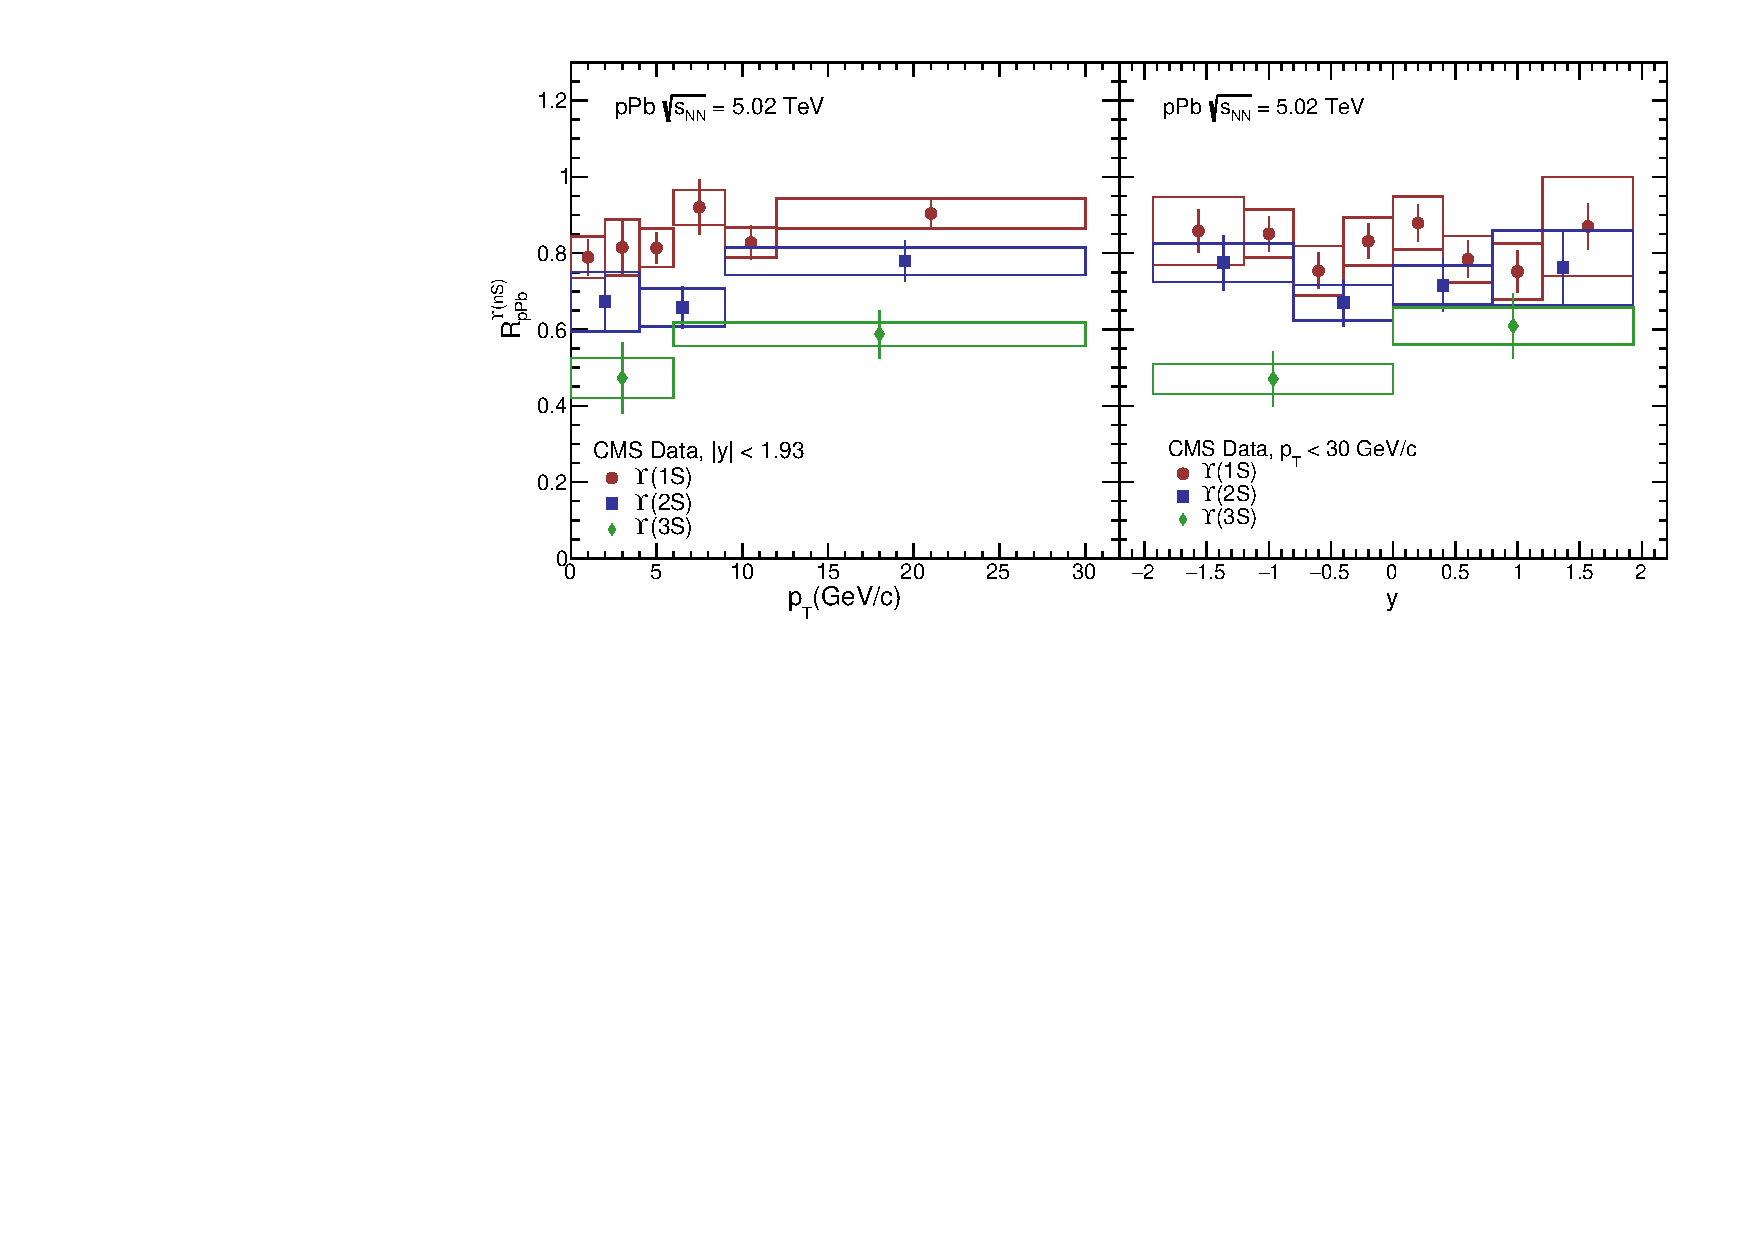
\includegraphics[width=0.99\textwidth]{Figures/Fig13_LHC_YnSRPPbPtRap.pdf}
     \caption{(Color online) The $\Upsilon$(nS) nuclear modification factor, $R_{pA}$,
      (a) as a function of transverse momentum $p_{T}$
    and (b) as a function rapidity in pPb colisions at 5.02 TeV measured by CMS~\cite{CMS:2022wfi}
  }
  \label{fig:LHCpPb5}
\end{figure}




Figure~\ref{fig:LHCpBPbPb} shows the $\Upsilon$(nS) nuclear modification factors,
    $R_{pA}$~\cite{CMS:2022wfi} and $R_{AA}$~\cite{CMS:2018zza}
 at 5.02 TeV measured by CMS.
 It is observed that Upsilon states are suppressed in both pPb and PbPb collisions
 though the suppression is many times more in PbPb collisions. There are
 final state effect in pPb collisions. 
    

\begin{figure}
\centering
  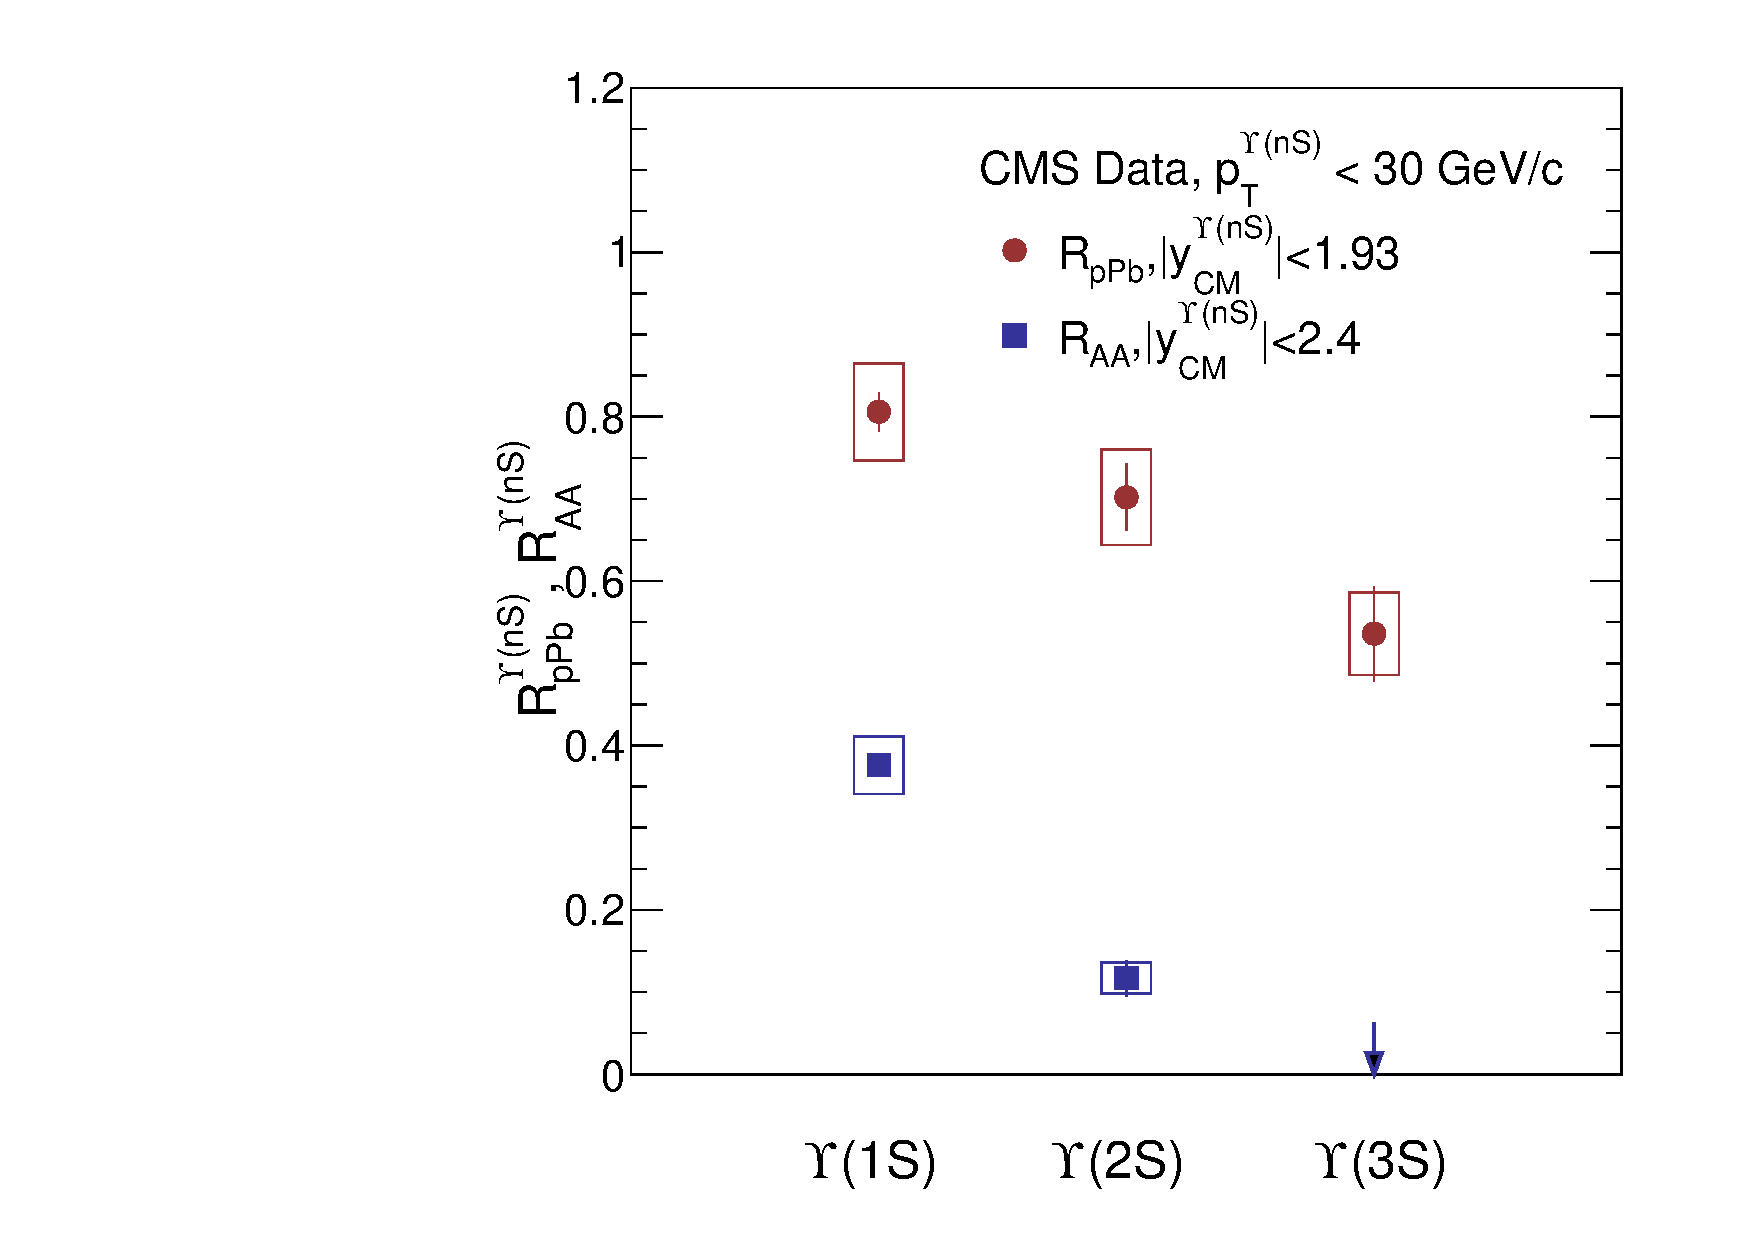
\includegraphics[width=0.60\textwidth]{Figures/Fig14_LHC_YnSRPPbRAAInt.pdf}
  \caption{(Color online) The $\Upsilon$(nS) nuclear modification factors,
    $R_{pA}$~\cite{CMS:2022wfi} and $R_{AA}$~\cite{CMS:2018zza}
    at 5.02 TeV measured by CMS.
  }
 \label{fig:LHCpBPbPb}
\end{figure}



  

